\documentclass[a4paper,12pt,twoside]{report}

% Import packages
\usepackage{acronym}
\usepackage{url}
\usepackage{cite}
\usepackage{listings}
\usepackage[pdftex]{graphicx}
\usepackage[hang,small,bf]{caption}
\usepackage{template/tum}
\usepackage{setspace}
\usepackage[german,english]{babel}
\usepackage{float}
\usepackage{floatflt}
\usepackage{fancyhdr}
\usepackage{color}
\usepackage{booktabs}
\usepackage[pdftex,bookmarks=true,plainpages=false,pdfpagelabels=true]{hyperref}
\usepackage{mdwlist}
\usepackage{enumerate}
\usepackage{array}
\usepackage{longtable}
\usepackage{listings}
\usepackage[utf8]{inputenc}
\usepackage[capitalize, noabbrev]{cleveref}

% Import additional settings
% this file can contain additional settings, that are specific to this thesis

% Add additional packages
\usepackage{microtype}

% Define a default path for graphics
%\graphicspath{{figures/}}



% Insert the template folder to the graphics path, so the faculty logo can always be imported, whether or not the author as specified a graphics path.
\makeatletter
	\providecommand*{\Ginput@path}{}
	\g@addto@macro\Ginput@path{{template/}{./}}
\makeatother

\begin{document}

	%
	\setlength{\evensidemargin}{22pt}
	\setlength{\oddsidemargin}{22pt}

	% Import some metadata about this thesis
	% define the type of the thesis. E.G.:
% - Master's Thesis
% - Bachelor's Thesis
\def\doctype{Bachelor's Thesis}

% state the faculty, to which this thesis is submitted. E.G.:
% - Informatics
% - Sport and Health Sciences
\def\faculty{Informatics}

% state the English title of the thesis
\def\title{Towards Design and Development of a Web Chatbot System for Early Detection of Neurodegenerative Diseases through Typing Behavior Analysis}

% state the German title of the thesis
\def\titleGer{Beitrag zur Entwurf und Entwicklung eines Web-Chatbot-Systems zur Früherkennung von neurodegenerativen Krankheiten durch Analyse des Tippverhaltens}

% state the professor, who is supervising the thesis. E.G.:
% - Prof. Bernd Brügge, Ph.D.
% - Prof. Dr. Stephan Jonas
\def\supervisor{Prof. Dr.-Ing. J org Ott}

% state the assistant, who helped supervising the thesis
\def\advisor{Yifan Yang, M.Sc.}

% state your own name
\def\author{Nicolas Othmar Theodarus}

% state the date, when this thesis is submitted
\def\date{03.03.2025}


	%
	\hypersetup{pdfborder={0 0 0}, pdfauthor={<author>}, pdftitle={<title english>}}
	\lstset{showspaces=false, numbers=left, frame=single, basicstyle=\small}

	% Number the introductory pages with letters
	\pagenumbering{alph}

	% Include a couple of introductory pages
	\thispagestyle{empty}

\vspace{4cm}
\begin{center}
\oTUM{4cm}\\ 
\vspace{5mm}     
\huge FAKULT{\"A}T F{\"U}R INFORMATIK\\ 
\vspace{0.5cm}
\large DER TECHNISCHEN UNIVERSIT{\"A}T M{\"U}NCHEN\\
\vspace{1mm}
\end{center}

\vspace{13mm}

\begin{center}
{\Large \doctype\ in \faculty}
\vspace{20mm}

\begin{spacing}{1.5}
{\huge\bf \title}\\%[3ex]
\end{spacing}

\vspace{15mm}
{\LARGE \author}

\vspace{10mm}

\begin{figure}[h!]
\centering

\includegraphics[width=4cm]{InformaticsLogo}
\end{figure}

\end{center}

	\thispagestyle{empty}

\vspace{8mm}
\begin{center}
\oTUM{4cm}

\vspace{5mm}     
\huge FAKULT{\"A}T F{\"U}R INFORMATIK\\ 
\vspace{0.5cm}
\large DER TECHNISCHEN UNIVERSIT{\"A}T M{\"U}NCHEN\\
\end{center}

\vspace{5mm}

\begin{center}
{\Large \doctype\ in \faculty}
\vspace{8mm}

\begin{spacing}{1.3}
{\LARGE \title}\\
\vspace{8mm}

{\LARGE \titleGer}\\
\vspace{8mm}
\end{spacing}

\begin{tabular}{ll}
\Large Author:     & \Large \author     \\[2mm]
\Large Supervisor: & \Large \supervisor \\[2mm]				
\Large Advisor:	   & \Large \advisor    \\[2mm]
\Large Date:       & \Large \date
\end{tabular}

\vspace{1mm}

\begin{figure}[hb!]
\centering

\includegraphics[width=4cm]{InformaticsLogo}
\end{figure}

\end{center}

	\newpage
	\thispagestyle{empty}
	\mbox{}
	\clearpage
\thispagestyle{empty}
\vspace*{0.8\textheight}
\noindent
I assure the single handed composition of this bachelor thesis only supported by declared resources,

\vspace{15mm}
\noindent
Munich, \date \hspace{\stretch{1}} \author
\newpage



	\newpage
	\thispagestyle{empty}
	\mbox{}
	\chapter*{Acknowledgements}

I am extremely grateful to my supervisor, Yifan Yang, M.Sc. and Leon Nissen, M.Sc., for their guidance and support throughout my research.
I also could not have completed this work without the help of Prof. Dr. rer. medic. Stephan Jonas and the whole insitute of digital medicine team of Bonn University Hospital, whose resources and assistant were invaluable to me.
Additinonally, I would like to extend my gratitude towards technical university of Munich and Prof. Dr.-Ing. J org Ott, for providing me with the opportunity to conduct this research.				

Special thanks to my family and friends for their support and encouragement throughout my studies.
Their unwavering belief in me has been a constant source of motivation.
Lastly, I would be remiss in not mentioning the correspondents who used my application and allowed me to collect data for this research.

	% Number the overview pages with roman numbers
	\pagenumbering{roman}

	% Include the abstract in English and German
	\selectlanguage{english}
	\begin{abstract}
		%abstract english

% \textit{Note: you will write two abstracts for your thesis}

% \textit{
% 	\textbf{the first abstract} will be written at the very beginning of your thesis.
% 	It shall contain a description of the problem, you want to solve, and present a plan how you plan to address that problem.
% }

% \textit{
% 	The purpose of this first abstract is to specify the topic of the thesis.
% 	It is meant to reflect to the supervisor, how you have understood the task.
% 	Also, it gives you the opportunity to define a focus or to add topics, that you are interested in, to the scope of your thesis.
% }

% \textit{\textbf{1. paragraph:} What is the motivation of your thesis? Why is it interesting from a scientific point of view? Which main problem do you like to solve?}

% \textit{\textbf{2. paragraph:} What is the purpose of the document? What is the main content, the main contribution?}

% \textit{\textbf{3. paragraph:} What is your methodology? How do you proceed?}

Neurodegenerative diseases are chronic conditions that destroy and damage part of nervous system of the sufferer over time, especially the brain. 
This diseases pose a significant challenge for general public health, since the damages are permanent and incurable. 
This condition happens mainly on elderly people, given that aging is the greatest risk factor. 
Moreover, early detection of these diseases are inefficient, impractical and only have minuscule success percentage. 
There is a need for better detection methods that are cost-effective, user-friendly and accurate.

This thesis aims to pave the way of developing the aforementioned better detection methods.
In this thesis, a mobile optimized web application to gather typing data from users of different age groups will be developed. 
A clean and robust architecture structure is utilised to guarantee reliability, scalability and maintainability. 
It should also be ensured that the application is able to effectively process and save the collected data, so that the data can be used for research purposes.
After this thesis, the application can hopefully be developed further with more advanced features in the future. 
An example of such additional feature would be an analysis functionality, where typing behaviour data of a person can instantly be analysed with a click of a button.

Analysis of the data is done with the goal to find statistical properties.
These statistical propertiess hopefully can be used to differentiate between different age groups.
Building a robust application that can collect typing data from its users, and then analysing said data to find interesting properties, is the main contribution of this thesis. 
The conclusion derived from this thesis could give insight into the feasibility of utilising biomarkers to effectively monitor health condition of the user.
Specifically, the author hopes that this findings would be beneficials for research on detecting early signs of neurodegenerative disorders effectively with a simple method of collecting typing pattern data.
	\end{abstract}
	\clearpage
	
	\selectlanguage{german}
	\begin{abstract}
		%abstract german
\textit{Note: Insert the German translation of the English abstract here.}

	\end{abstract}
	\clearpage
	\selectlanguage{english}

	% Create a table of contents
	\tableofcontents
	\clearpage
	\clearpage

	% Include the list of acronyms and abbreviations
	\begin{acronym}
\acro{AD}{Alzheimer's Disease}
\acro{PD}{Parkinson's Disease}
\acro{UI}{user interface}
\acro{DAO}{Data Access Object}
\acro{DTO}{Data Transfer Object}
\acro{LLM}{large language model}
\end{acronym}
	\clearpage
	\clearpage
	
	% Include the outline of your thesis
	\phantomsection
\chapter*{Outline of the Thesis}

%--------------------------------------------------------------------

\noindent {\scshape Chapter 1: Introduction}  \vspace{1mm}

\noindent  Text \\

\noindent {\scshape Chapter 2: Background}  \vspace{1mm}

\noindent  Text \\

\noindent {\scshape Chapter 3: Related Work}  \vspace{1mm}

\noindent  Text \\

\noindent {\scshape Chapter 4: Requirements Elicitation}  \vspace{1mm}

\noindent  Text \\

\noindent {\scshape Chapter 5: System Design}  \vspace{1mm}

\noindent  Text \\

\noindent {\scshape Chapter 6: Case Study/Evaluation}  \vspace{1mm}

\noindent  Text \\

\noindent {\scshape Chapter 7: Summary}  \vspace{1mm}

\noindent  Text \\

	% Number the content of the thesis in Arabic numbers
	\pagenumbering{arabic}

	%
	\fancyhead{}
	\pagestyle{fancy}
	\fancyhead[LE]{\slshape \leftmark}
	\fancyhead[RO]{\slshape \rightmark}
	\headheight=15pt

	% Include all the chapters
	% include the files from the chapters folder here
\chapter{Introduction}

% \textit{Note: Introduce the topic of your thesis, e.g. with a little historical overview.}

\ac{AD} and \ac{PD}, are chronic and progressive neurodegenerative diseases that primarily affect the nervous system.
This diseases lead to the degeneration of motoric and cognitive abilities.
These diseases are often irreversible and incurable, posing significant public health challenges.
As populations age, the risk of such disorders increase substantially, making early detection crucial.

Historically, the diagnosis of neurodegenerative diseases has been done throuh clinical observations, imaging, and biomarkers.
Even though medical technologies have improved significantly over the years, there are still many challenges for early diagnosis.
One of the main reason for this is because neurodegenerative diseases develop gradually over time.
Early symptoms of these diseases can easily be overlooked or mistaken as normal aging \cite{manera2023}.
As a result, these early symptons are often ignored until the disease itself has reached a critical stage, where the chance of treatment declines significantly. 
Furthermore, current diagnostic methods are expensive, invasive, and often inaccessible to a large portion of the population.

A better method is obviously needed to battle these insidious diseases.
The rise of technologies such as smartphones open up new possibilities for early detection of these conditions.
One example of such possibility is to utilise a phone application as a mean to detect early neurodegenerative diseases.
Studies have shown that one of the effect of these diseases, i.e. impairments of motoric functions, will be reflected on how a person types \cite{mcisaac2023}.
This changes in typing behaviors, such as typing speed, accuracy, and keystroke patterns can then be recorded by the application.
The data acquired by this application might be able to be used to analyse early symptons of \ac{AD} and \ac{PD}.

\section{Problem}

% \textit{Note: Describe the problem that you like to address in your thesis to show the importance of your work.
%  Focus on the negative symptoms of the currently available solution.
% }

It is clear from the facts mentioned above, that neurodegenerative diseases are problems that need to be addressed.
World Health Organisation estimates that there are approximately 50 million people worldwide affected by these disorders.
Most of the sufferer are elderly, since age is one of the main risk factor.
As the most common neurogedenerative disorder, \ac{AD} still lacks an effective cure.
It is even harder to treat the more progressive the disease progress.
That is why the importance of an effective way to diagnose the disease early cannot be overstated. 
In the current state, however, misdiagnosis rates are still high, reaching up to 20\% \cite{Fischer2017}.
Not only that, current diagnostic methods are either invasive, costly, or impractical for widespread use.

Similarly, \ac{PD}, the second most common neurodegenerative disorder, has no cure and limited treatment options. 
For this disease too an effective mean for early diagnosis is of utmost importance.
Since with a successful early detection, the progression of the disease can be slowed significantly, improving the quality of life of patients greatly.
The current diagnostic methods for this disease, however, rely mostly on the observation of changes of motoric symptoms.
These methods, as previously discussed, are unreliable for many reasons.

In both conditions, early intervention can significantly improve patient outcomes, but existing diagnostic tools fail to provide a practical and accurate solution for early detection. 
There is a pressing need for non-invasive, cost-effective, and widely accessible methods to detect early signs of neurodegenerative diseases before the onset of significant symptoms.

\section{Motivation}

% \textit{Note: Motivate scientifically why solving this problem is necessary.What kind of benefits do we have by solving the problem?}

The motivation for this thesis comes from the urgent need to find better diagnostic methods for neurodegenerative diseases. 
Finding methods to effectively detect early these diseases would significantly improve general public health.
Early detection allows for earlier interventions, which will then slow the progression of the diseases.
This would improve treatment outcomes, and ultimately reduce the burden on healthcare systems.

From a scientific point of view, the research on using digital biomarker, i.e. typing pattern, as a mean to detect neurodegenerative diseases is underexplored.
This research could give insights into how effective common tools and activities can be used to improve public health.
Typing has became a common daily activity for most modern human, especially with the widespread use of smartphones and chat applications.
This means that it can be a low-cost and non-invasive method to detect subtle motoric or cognitive impairments.
In the most ideal case, the subject would not even notice that they are being monitored for these diseases and can go on about enjoying their daily lives.

Taking advantage of these common daily activities could help reduce the risk of neurodegenerative diseases, by diagnosing them as early as possible.
Furthermore, these methods would also be accessible to people that lives in less developed countries with less developed medical technologies.
This would ensure equal chances to fight against these neurodegenerative diseases.
By developing a mobile-optimized web application that can collect and analyze typing data in real time, it would also become easier to monitor people's condition.
Especially the condition of those that are more prone to this diseasesm, i.e. the elderly.

\section{Objectives}

% \textit{Note: Describe the research goals and/or research questions and how you address them by summarizing what you want to achieve in your thesis, e.g. develping a system and then evaluating it.}

Developing a web-based chat application that can capture and analyze typing behavior for early detection of neurodegenerative diseases is an ambitious goal.
That goal is unfortunately not in the scope of this thesis.
Collecting pathological data that is required for the aforementioned goal requires a lot of process and time, which does not align with the time limitation of this thesis.
Another more suitable objective for this thesis would be to explore whether it is possible to determine the age of a user based on their typing patterns.
The author believe that this thesis will pave the way for a more advanced research on this matter.
This thesis wants to show that typing pattern can be used to identify the characteristics of the user, in this case, the age group.

Specifically, this thesis aims to:
\begin{enumerate}
    \item Develop mobile-optimized chat application that collects the user's typing data.
    The main focus is to collect samples from individuals across different age groups.
    \item Practice clean architecture and secure coding practices to make sure the application is reliable, scalable, and maintainable. 
    The chat application will be designed to be user-friendly for all age groups, specifically the elderly.
    \item Analyze the gathered typing behavior data to identify patterns or statistical distributions that may correlate with the user's age. 
    Metrics such as typing speed, keystroke intervals, and error rates will be examined to determine if they can give indication of the user's age group.
    \item Evaluate the accuracy of using typing behavior as a predictor of age.
    The identified patterns need to be consistent enough to be able to reliably be used to estimate the user's age group.
\end{enumerate}

The goal of this thesis is to research the feasibility of using data of typing behavior gathered by the application to profile the user in an age group.
If this is achieved, the author hopes that this could give insights that would be valuable for future research in user profiling or cognitive assessments.
The application could also be further developed to be able to analyse more complex matters, such as early signs of neurodegenerative disorders.
Another possible improvement would be adding real-time analysis of the typing pattern and integration with healthcare systems.
This would be beneficials for patients and clinicians alike.
\chapter{Background}

% \textit{Note: Describe each proven technology / concept shortly that is important to understand your thesis. Point out why it is interesting for your thesis. Make sure to incorporate references to important literature here.}

\section{Mobile-Optimized Applications and Accessibility for Elderly Users}

It is crucial that the application is both mobile-optimized and also accessible to elderly users.
Since the author wants to use data of people typing on their smartphones, the application needs to be mobile-optimized.
Mobile-optimized application ensures that the data gathered by this application captures typing pattern of its users correctly.
Irregularities, such as typing mistakes or longer typing interval, should not be caused by the difficulty of using this application.
Instead this irregularities should reflect human error, that most likely to happens more frequently with older subjects.
Among other thigs, the \ac{UI} design of the application should be clean and minimalist, focusing on essential features and contents.
Unnecessary elements and visual clutters should be removed to create an intuitive \ac{UI} that is easy to navigate on smaller screens.
Since there are many types and sizes of smartphones, it is also important to build a responsive web application that is able to adjust to common screen sizes.

The application also need to be accessible for elderly users.
This is done to prevent a false positive condition, where significantly more typing errors happen on elderly subjects because of the difficulty of using the application.
Designing an accessible \ac{UI} for the elderly requires some considerations as suggested by Gomez-Hernandez et. al. in their research in 2023\cite{hernandez2023}:
\begin{enumerate}
    \item \textbf{Bigger Interactive Elements:} The size of interactive elements, such as buttons and forms, need to be bigger to make them more accessible.
    This improvement could help with possible vision or motoric impairments.
    \item \textbf{High contrast:} Another method to help with vision impairment.
    This could help increase readability.
    \item \textbf{Font Selection:} The font used should be easily readable, especially on smaller screens.
    \item \textbf{Spacing:} Enough spacing should be added to improve readability und user experience.
    \item \textbf{Apropriate color choices}: Avoiding colors like blue, violet, and green, and yellow, which can become harder to distinguish with age due to shifts in color perception.
    \item \textbf{Centralized content}: Placing key elements in the center of the interface to make them easier to find and interact with.

\end{enumerate}


\section{Backend Architecture: Java Spring Boot}
On the backend side of the application, Java Spring Boot framework is utilised to manage and process data that are sent by the frontend of the application.
The Spring Framework is an application framework and inversion of control container for the Java programming language.
Spring Boot is an open-source Java framework for applications based on Spring to help project startup and management easier.
This framework provides libraries that help to develop a scalable, maintainable and secure web applications.
It is important to develop the application in this manner so that new features and improvement could easily be added during or after the writing of this thesis.
If the occassion arises, this application would also be ready to be reused for a possible follow-up research on this topic.

Spring Boot provides functionalities that help to ensure clean architecture and adherence to coding principles, such as DRY (Don't Repeat Yourself).
Another important feature provied by Spring Boot is RESTful services, that support separation of the client and the server.
Other than aiding on building a clean architecture, RESTful services also further ensure the possibility of reusing the code for further researches.
This application uses \ac{DAO} and \ac{DTO} patterns to manage data efficiently.
This separation of concerns between \ac{DAO} and \ac{DTO} adheres to clean architecture principles, improving maintainability and testability.

\section{Database Management: PostgreSQL}
PostgreSQL is an open-source, object-relational database system known for its scalability, reliability and support for complex queries.
These attributes make PostgreSQL ideal for storing a huge amount typing data and keystroke logs.
Features such as JSONB data type that is offered by PostgreSQL also help to simplify data processing and storing, especially data of keystroke logs. 
Another reason why PostgreSQL is used in this project is its indexing and search capabilities.
This will be crucial for fast retrieval of user data, allowing efficient typing pattern analysis that would be useful if instant analysis feature is ever built.

\section{Large Language Models: Llama3}
The Llama3 is the latest \ac{LLM} develop by Meta inc.
In addition to Llama3's impressive performance compared to other \ac{LLM}s, Llama3 is multilingual and can support both english and german language well.
This makes Llama3 the perfect language model to use for this thesis.
In this thesis, Llama3 will be used to chat with the users in real-time.
The language model is prompted to try to get as much response from the users as possible, so that the typing data can be collected.

It is interesting to see whether \ac{LLM}s such as Llama3 would be able to also analyze the users' typing data.
It can potentially help identify changes and irregularities in typing pattern that might indicate the age of the user.
If this is possible, a real-time analysis of the typing pattern might be able to be implemented with the help of language models.
This topic is, however, not in the scope of this thesis and is only a possible future research.

\section{Containerization: Docker}
To further promotes the scalability of the application, the author utilizes Docker.
Docker is a platform for delivering software in packages called containers.
Containerization is an important part of deploying a scalable application across various environments.
Docker allows applications to be deployed separately (frontend, backend, database and \ac{LLM}) in their own separated containers.
This makes it easier for the application to be reused and rebuild in other environments, such as on the university servers.

\section{Pattern Recognition and Analysis of Typing Pattern}

After the data is collected, the next step is to analyze the data.
The main purpose of this analysis is to find patterns in the typing behavior of the users that might correlate with their age group.
Statistical analysis will be used to find correlation between typing metrics and age group, such as by finding mean and standard derivation of duration between keystrokes and error rates.
This analysis will be done in three evaluations.

In the evaluation, the data will be truncated to eliminate outliers.
The first truncation will be done by excluding duration between keystrokes that are more than 5 seconds.
This is done to eliminate the possibility of the user being distracted or leaving the application.
The second truncation will be done by removing the one-percenth quantile (\textless1\% and \textgreater99\%) of duration between keystrokes.
This is done to remove outliers of the data.

In a third evaluation, the \ac{IQR} method will be used to find outliers of the data.
The \ac{IQR} is a measure of statistical dispersion, often used to detect outliers in data. 
It represents the range within which the central 50\% of the data lies.
First, similar to the previous two evaluations, the data will be truncated to exclude duration between keystrokes that are more than 5 seconds.
Then, the \ac{IQR} will be calculated and used to truncated the outliers of the data.

\section{Privacy in Data Collection}

Anonimity and privacy of the users are insured by not collecting any personal data, other than the age of the user.
The application will not ask for any personal information, such as name, address, or phone number.
This, combined with the fact that the application can be accessed by multiple users at the same time, ensures that the data collected is anonymous.

\chapter{Related Work}

\textit{Note: Describe related work regarding your topic and emphasize your (scientific) contribution in \textbf{contrast} to existing approaches / concepts / workflows. Related work is usually current research by others and you defend yourself against the statement: ``Why is your thesis relevant? The problem was already solved by XYZ.'' If you have multiple related works, use subsections to separate them.}

\chapter{Requirements Elicitation}

\textit{Note: This chapter follows the Requirements Analysis Document Template in \cite{bruegge2004object}. 
\textbf{Important:} Make sure that the whole chapter is independent of the chosen technology and development platform. The idea is that you illustrate concepts, taxonomies and relationships of the application domain independent of the solution domain!
Cite \cite{bruegge2004object} several times in this chapter.}

\section{Overview}

\textit{Note: Provide a short overview about the purpose, scope, objectives and success criteria of the system that you like to develop.}

\section{Current System}

\textit{Note: This section is only required if the proposed system (i.e. the system that you develop in the thesis) should replace an existing system.}

\section{Proposed System}

\textit{Note: If you leave out the section ``Current system'', you can rename this section into ``Requirements''.}

\subsection{Functional Requirements}

\textit{Note: List and describe all functional requirements of your system. Also mention requirements that you were not able to realize. The short title should be in the form ``verb objective''}

\begin{itemize}
\item [FR1] \textbf{Short Title}: Short Description.
\item [FR2] \textbf{Short Title}: Short Description.
\item [FR3] \textbf{Short Title}: Short Description.
\end{itemize}

\subsection{Nonfunctional Requirements}

\textit{Note: List and describe all nonfunctional requirements of your system. Also mention requirements that you were not able to realize. Categorize them using the FURPS+ model described in \cite{bruegge2004object} without the category \textbf{functionality} that was already covered with the functional requirements.}

\begin{itemize}
\item [NFR1] \textbf{Category}: Short Description.
\item [NFR2] \textbf{Category}: Short Description.
\item [NFR3] \textbf{Category}: Short Description.
\end{itemize}

\section{System Models}

\textit{Note: This section includes important system models for the requirements analysis.}

\subsection{Scenarios}

\textit{Note: If you do not distinguish between visionary and demo scenarios, you can remove the two subsubsections below and list all scenarios here.}

\subsubsection{Visionary Scenarios}

\textit{Note: Describe 1-2 visionary scenario here, i.e. a scenario that would perfectly solve your problem, even if it might not be realizable. use our scenario description template in form of a table.}

\subsubsection{Demo Scenarios}

\textit{Note: Describe 1-2 demo scenario here, i.e. a scenario that you can implement and demonstrate until the end of your thesis. use our scenario description template in form of a table.}

\subsection{Use Case Model}

\textit{Note: This subsection should contain a UML Use Case Diagram including roles and their use cases. You can use colors to indicate priorities. Think about splitting the diagram into multiple ones if you have more than 10 use cases.
\textbf{Important:} Make sure to describe the most important use cases using the use case table template. Also describe the rationale of the use case model, i.e. why you modeled it like you show it in the diagram.}

\subsection{Analysis Object Model}

\textit{Note: This subsection should contain a UML Class Diagram showing the most important objects, attributes, methods and relations of your application domain including taxonomies using specification inheritance (see \cite{bruegge2004object}). Do not insert objects, attributes or methods of the solution domain.
\textbf{Important:} Make sure to describe the analysis object model thoroughly in the text so that readers are able to understand the diagram. Also write about the rationale how and why you modeled the concepts like this.}

\subsection{Dynamic Model}

\textit{Note: This subsection should contain dynamic UML diagrams. These can be a UML state diagrams, UML communication diagrams or UML activity diagrams.\textbf{Important:} Make sure to describe the diagram and its rationale in the text. \textbf{Do not use UML sequence diagrams.}}

\subsection{User Interface}

\textit{Note: Show mockups of the user interface of the software you develop and their connections / transitions. You can also create a storyboard. \textbf{Important:} Describe the mockups and their rationale in the text.}

\chapter{System Design}

% \textit{Note: This chapter follows the System Design Document Template in \cite{bruegge2004object}. 
% You describe in this chapter how you map the concepts of the application domain to the solution domain. Some sections are optional, if they do not apply to your problem.
% Cite \cite{bruegge2004object} several times in this chapter.}

\section{Overview}

% \textit{Note: Provide a brief overview of the software architecture and references to other chapters (e.g. requirements analysis), references to existing systems, constraints impacting the software architecture.}

This chapter explains the decision regarding the architecture design of the application.
Design of the architecture will be largely based on bridging the conceptual understanding of the application with the concrete technical solution.
Requirements of the system and existing constraints are also the main deciding factors of the architecture design.
The system aims to address the nonfunctional requirements of the application, such as performance and usability, which were mentioned in earlier chapters.
Based on Bruegge and Dutoit's template \cite{bruegge2004object}, the structure of the system is divided into logical components and subsystems.

\section{Design Goals}

% \textit{Note: Derive design goals from your nonfunctional requirements, prioritize them (as they might conflict with each other) and describe the rationale of your prioritization. Any trade-offs between design goals (e.g., build vs. buy, memory space vs. response time),
% and the rationale behind the specific solution should be described in this section}

Design goals of the system are derived from nonfunctional requirements.
Because of constraints such as time, some of the nonfunctional requirements might not be fulfilled.
The design goals are prioritized based on the importance of the nonfunctional requirements.
Design goals of the system are as follows:

\begin{itemize} 
    \item \textbf{Usability and Accessibility}:
    One of the most important goal of the system is to be usable and accessible for the elderly.
    For this goal, the application is designed to be user-friendly for all age groups, specifically the elderly.
    The UI should be intuitive and easy to use.
    This is achieved through big buttons, clear visual indicators and enough spacing between elements.
    Design of the application should be accessible for the elderly with features such as large fonts, enough spacing, and clear visual indicators. 
    This design goal is purely achieved through the frontend of the application.
    As such, the only limiting constraint is the time and resources available to develop the frontend.

    \item \textbf{Reliability}: 
    Another most important goal of the system is reliability of the system.
    Reliability here means that the system should be able to accurately gather, process and store the typing pattern data.
    Since a faulty or inaccurate data could lead to wrong conclusion, the system should be able to minimize the inaccuracy of the data.
    Both the frontend and backend of the application play a role in achieving this goal.
    The frontend should be able to accurately capture the typing pattern data, especially the attribute timeSinceLastKey.
    This attribute shows information about the time difference between the last key press and the current key press.
    For this purpose, the built in JavaScript function Date.now() is used.

    \item \textbf{Performance}: 
    Recording the typing pattern data in real-time is not a performance heavy task.
    This function can easily be achieved by creating an array of keystroke data that is updated every time a key is pressed.
    The main performance issue of the application is waiting for the \ac{LLM} to respond to the user's message.
    The \ac{LLM} is instructed to try to get as much response from the users as possible, so that more typing data can be collected.
    This leads to a longer waiting time for the user to get a response, since the longer the response from the \ac{LLM}, the longer it will take for the \ac{LLM} to finish the response.
    One of the possibility of solving this problem would be to stream the response from the \ac{LLM}.
    Stream will allow the user to see response from the \ac{LLM} in chunks, instead of waiting for the whole response to be finished.
    Unfortunately this feature is not yet implemented in this application due to time constraints.

    \item \textbf{Privacy}: 
    An application that concerns itself with collecting sensitive user data should be secure and able to keep the data private.
    In this application, a chat session can be accessed by inputting a session ID.
    As a measure to increase privacy, each chat session can be made inaccessible by changing an attribute in the database.
    When a user tries to access a chat session that is already closed, the application will return an error message.
    Another important factor regarding privacy is anonimity.
    The only information about the user that is saved in the database is the user's age.
    If another user tries to access chat session of another user that is not yet deactivated, the message history will be shown.
    However, the user's age will not be shown.

    \item \textbf{Adaptability}: 
    Adaptability means the ease with which a system may be modified to fit changed requirements or environment.
    Adaptability of the system can be divided into two parts: adaptability of the frontend and adaptability of the backend.
    The frontend of the application is designed to be easily modifiable by utilising component based design of the React library.
    Adaptability of the backend is ensured by utilising concepts such as encapsulation and modularity.
    The backend is divided into several classes, each responsible for a specific task.
    This allows for easy modification of the backend, since each class can be modified without affecting the other classes.
    The only limiting factor for adaptability is the time and resources available to modify the system.
    Docker is used to containerize the application, which allows for easy deployment and scaling of the application.

\end{itemize}
    

\section{Subsystem Decomposition}

% \textit{Note: Describe the architecture of your system by decomposing it into subsystems and the services provided by each subsystem. Use UML class diagrams including packages / components for each subsystem.}

The system is divided into two main subsystems: the frontend and the backend.
The frontend is responsible for capturing the typing pattern data and displaying the chat interface.
The backend is responsible for processing the typing pattern data and generating a response from the \ac{LLM}.

\subsection{Frontend}

\subsubsection{User Interface}

\begin{figure}[h!]
    \centering
    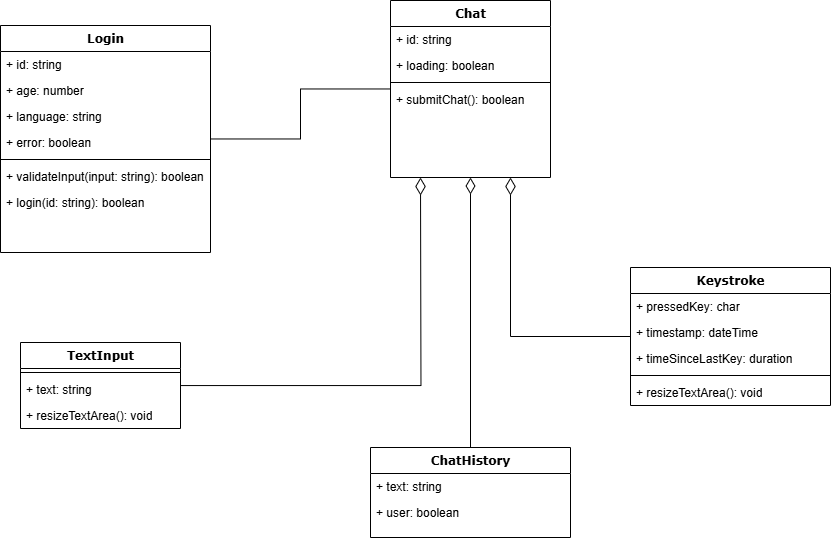
\includegraphics[width=13cm]{class_frontend.png}
    \caption{UML class diagram of the frontend architecture of the user interface.}
    \label{class_frontend}
\end{figure}

The frontend of the application of the user interface can be divided into two main components: the login component and the chat component.
Figure~\ref{class_frontend} shows the UML class diagram of the frontend architecture of the user interface.
The main purpose of the login page is to initialise the chat session and validate the user's input.
User inputs their age, the session ID, and the language to chat with the \ac{LLM}.
English and german are the two possible languages that the user can choose.

In the login page, the user can click the "Login" button to start the chat.
After this button is clicked, both the session ID and the user's age will first be validated.
On the frontend side, the session ID is validated by checking whether the session ID has 6 digits.
The user's age is validated by checking whether the user's age is a number and whether the user's age is between 1 and 99.
If the validation is successful, the data will be sent to the backend.
On the backend side, the session ID is validated by checking whether the session ID is alredy deactivated.
The deactivated attribute is a boolean attribute in the database that can be managed either through the admin interface or by directly changing the value in the database.

In the chat page, the user can see the chat history and type a message.
Directly after the user pass the login page, the user will be greeted by the \ac{LLM}.
This initial message from the \ac{LLM} is actually a default message set on the frontend.
This is done to remove the initial loading time of the \ac{LLM} response.
At the same time, the backend will boot up the \ac{LLM} by sending the initial prompt.
This makes it so that while the user thinks about the response to the initial message, the \ac{LLM} can load.
Without this feature, the user would have to wait for the \ac{LLM} to load before the user can see the initial message.

While the user is typing, the frontend will capture the typing pattern data.
Each keypress made by the user is recorded and stored in an array.
After the user presses the "Enter" key, the array of typing pattern data will be sent to the backend as shown below:

\begin{verbatim}
    [
      {
        "timestamp": "2024-10-29T13:40:35.966Z", 
        "pressedKey": "i", 
        "timeSinceLastKey": 0.0
      },
      {
        "timestamp": "2024-10-29T13:40:36.123Z", 
        "pressedKey": "m", 
        "timeSinceLastKey": 157.0
      }
      {
        "timestamp": "2024-10-29T13:40:36.330Z", 
        "pressedKey": " ", 
        "timeSinceLastKey": 207.0
      }
      {
        "timestamp": "2024-10-29T13:40:36.447Z", 
        "pressedKey": "f", 
        "timeSinceLastKey": 117.0
      }
      {
        "timestamp": "2024-10-29T13:40:36.504Z", 
        "pressedKey": "i", 
        "timeSinceLastKey": 57.0
      }
      {
        "timestamp": "2024-10-29T13:40:36.592Z", 
        "pressedKey": "n", 
        "timeSinceLastKey": 88.0
      }
      {
        "timestamp": "2024-10-29T13:40:36.701Z", 
        "pressedKey": "e", 
        "timeSinceLastKey": 109.0
      }
    ]
    \end{verbatim}

\subsubsection{Admin Interface}

\begin{figure}[h!]
    \centering
    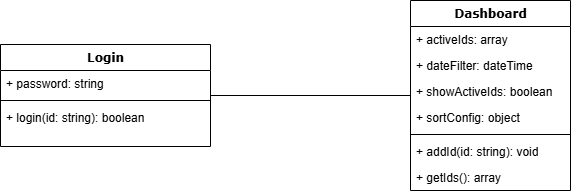
\includegraphics[width=13cm]{class_frontend_admin.png}
    \caption{UML class diagram of the frontend architecture of the admin interface.}
    \label{class_frontend_admin}
\end{figure}

The admin interface is a separate component of the frontend that is only accessible by the admin.
Figure~\ref{class_frontend_admin} shows the UML class diagram of the frontend architecture of the admin interface.
This admin interface can also be divided into two main components: the login component and the dashboard component.
Login page of the admin interface is significantly simpler than the login page of the user interface.
The admin only needs to input the admin password to access the admin interface.
After the "Login" button is clicked, the inputted password will be checked against the password set in the backend of the application.

The dashboard component helps manage the chat sessions by providing these functionalities:
\begin{itemize}
    \item View the list of all initialised chat sessions or initialised chat sessions that are still active.
    \item Deactivate a chat session
    \item Initialise a new chat session by inputting the ID of the chat session
    \item Sort the chat sessions by added date, ID, or deactivated date to ease the process of finding a specific chat session
\end{itemize}

\subsection{Backend}

\subsubsection{Main Controller}

\begin{figure}[h!]
    \centering
    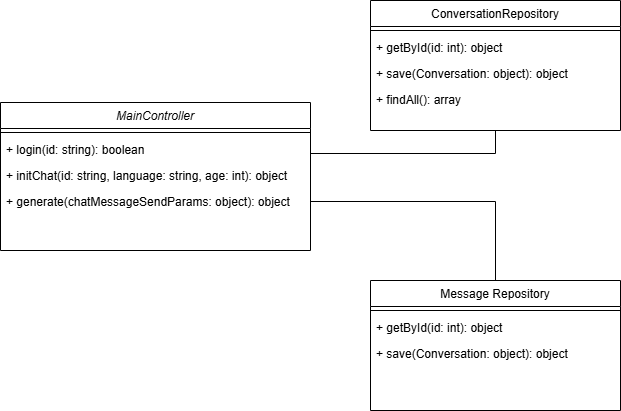
\includegraphics[width=13cm]{class_backend.png}
    \caption{UML class diagram of the backend architecture of the main controller.}
    \label{class_backend}
\end{figure}

The backend of the application can be divided into two main components: main controller and admin controller.
Figure~\ref{class_backend} shows the UML class diagram of the main controller.
This controller is responsible for handling login, initialisation of a chat session and getting a response from the \ac{LLM}.

\subsubsection{Admin Controller}

\begin{figure}[h!]
    \centering
    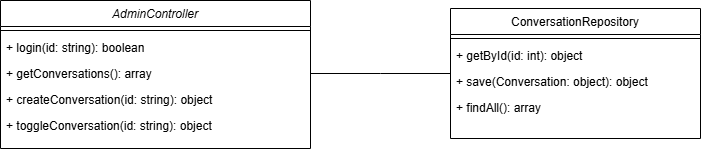
\includegraphics[width=13cm]{class_backend_admin.png}
    \caption{UML class diagram of the backend architecture of the admin controller.}
    \label{class_backend_admin}
\end{figure}

Figure~\ref{class_backend_admin} shows the UML class diagram of the admin controller.
This controller is responsible for handling the admin login and managing the chat sessions.
For managing the chat sessions, this controller provides these functionalities: get all chat sessions, deactivate and reactivate a chat session, and initialise a new chat session.

% \section{Persistent Data Management}

% \textit{Note: Optional section that describes how data is saved over the lifetime of the system and which data.
%  Usually this is either done by saving data in structured files or in databases.
%  If this is applicable for the thesis, describe the approach for persisting data here and show a UML class diagram how the entity objects are mapped to persistent storage.

% It contains a rationale of the selected storage scheme, file system or database, a description of the selected database and database administration issues.
% }

% \section{Access Control}

% \textit{Note: Optional section describing the access control and security issues based on the nonfunctional requirements in the requirements analysis.
%  It also describes the implementation of the access matrix based on capabilities or access control lists, the selection of  authentication mechanisms and the use of encryption algorithms.
% }

% \section{Global Software Control}

% \textit{Note: Optional section describing describing the control flow of the system, in particular, whether a monolithic, event-driven control flow or concurrent processes have been selected, how requests are initiated and specific synchronization issues}


% \section{Boundary Conditions}

% \textit{Note: Optional section describing the use cases how to start up the separate components of the system, how to shut them down, and what to do if a component or the system fails.}

\chapter{Evaluation}

% \textit{Note: If you did an evaluation / case study, describe it here.}

\section{Design}

% \textit{Note: Describe the design / methodology of the evaluation and why you did it like that. E.g. what kind of evaluation have you done (e.g. questionnaire, personal interviews, simulation, quantitative analysis of metrics, what kind of participants, what kind of questions, what was the procedure?}

The evaluation process was done to assess both the functional and non-functional requirements of the system.
This evaluation is done by processing the data collected from the users by the application.
The python library numpy and pandas are used to process the data.
Numpy is used to perform mathematical operations on the data and pandas is used to visualize the data.
If the system was able to collect and store data accurately, then the system is considered to be functioning correctly.
Whether the data being saved is accurate or not should be clear through the evaluation process.

\section{Objectives}

% \textit{Note: Derive concrete objectives / hypotheses for this evaluation from the general ones in the introduction.}

The data can be compared to the expected data to see if the system is functioning correctly.
An example of this would be to compare the average typing speed from the collected data and average typing speed data from other sources.
On average, the typing speed of a person on mobile devices is 36.2 \ac{WPM} with 2.3\% uncorrected errors \cite{Palin2019}.
This translate to 331.49 ms average duration between keystrokes, if we consider that on average, there are 5 characters per word.

Typing speed also varies depending ont he age of the user.
Age group 10-19 has the fastest typing speed with 39.6 \ac{WPM} and age group 50-59 has the slowest typing speed with 26.3 \ac{WPM} \cite{Palin2019}.
This translates to average speed between keystrokes of 303.03 ms for 39.6 \ac{WPM} and 456.65 ms for 26.3 \ac{WPM}.
This is the expected average duration between keystrokes for the data that has been collected by the application.

\section{Results}

% \textit{Note: Summarize the most interesting results of your evaluation (without interpretation). Additional results can be put into the appendix.}

\begin{table}[h]
    \centering
    \begin{tabular}{ccccc}
    \toprule
    \textbf{Age Group} & {Conversations} & Message Count & Message Length (Mean) \\
    \midrule
    0-24     & 7 & 26 & 19.77 \\
    25-39    & 9 & 39 & 53.59\\
    40-59    & 18 & 103 & 48.56\\
    60+      & 6 & 30 & 32.17 \\
    \bottomrule
    \end{tabular}
    \caption{Amount of unique conversations of each age groups.}
    \label{tab:unique_conversations}
\end{table}

\begin{figure}[h!]
    \centering
    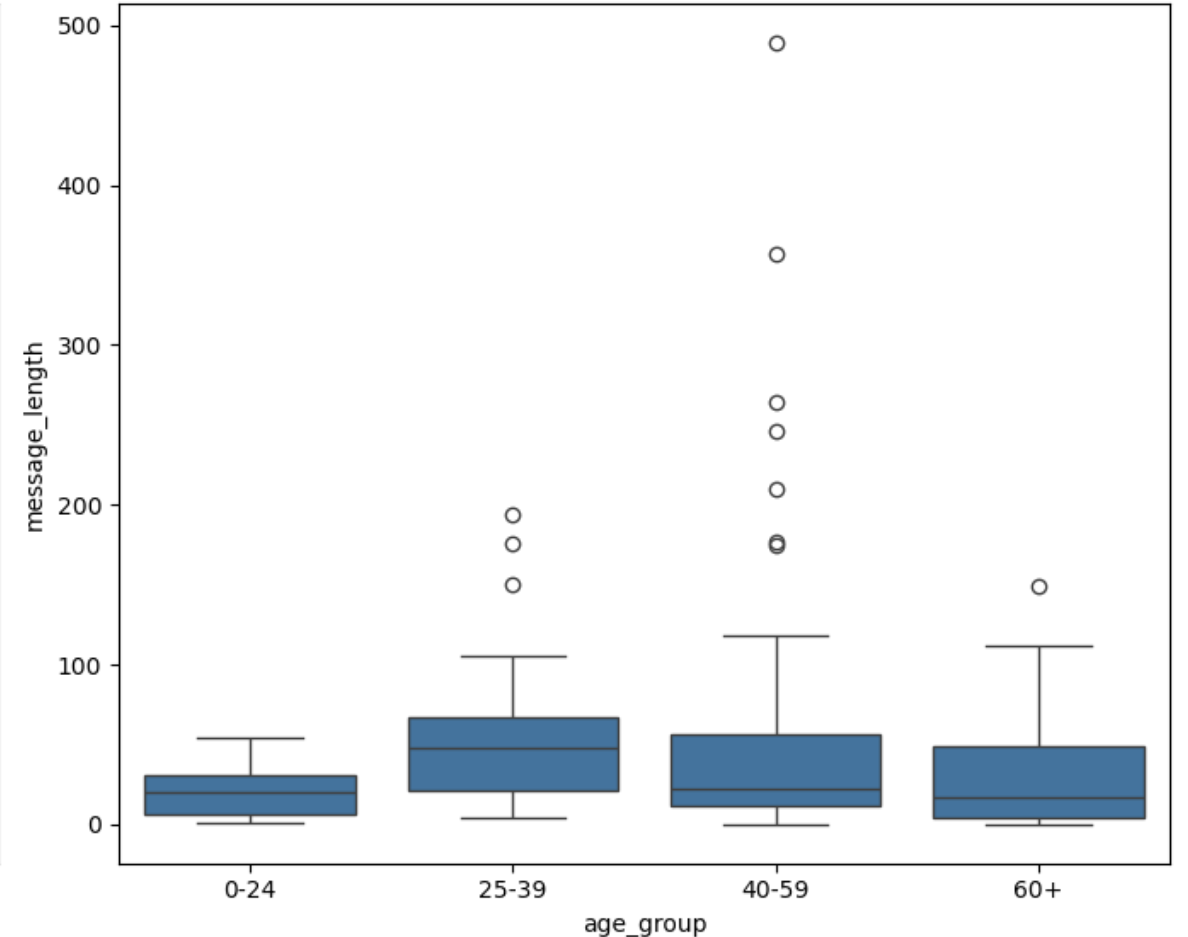
\includegraphics[width=13cm]{message_length.png}
    \caption{Box plot of message length of each age group.}
    \label{box_plot_message_length}
\end{figure}


Table \ref{tab:unique_conversations} shows the number of unique conversations, number of messages sent and the average length of the message sent.
In total, the application managed to gather data from 40 unique conversations.
Age group 40-59 has the most unique conversations with 18 conversations and most message sent with 103 messages.
Meanwhile age group 60+ has the least unique conversations with 6 conversations.
The least amount of messages sent is by age group 0-24 with 26 messages.

Regarding message length average, age group 25-39 has the longest message length average with 53.59 characters.
Age group 40-59 has the second longest message length average with 48.56 characters.
Age group 0-24 has the shortest message length average with 19.77 characters.

\begin{table}[h]
    \centering
    \begin{tabular}{ccccc}
    \toprule
    \textbf{Age Group} & Backspace Percentage (Mean, \%) \\
    \midrule
    0-24     & 6.00 \\
    25-39    & 6.63 \\
    40-59    & 15.93 \\
    60+      & 3.29 \\
    \bottomrule
    \end{tabular}
    \caption{Average of backspace percentage of each age groups.}
    \label{tab:backspace_percentage}
\end{table}

Table \ref{tab:backspace_percentage} shows the average backspace percentage of each age group.
Backspace percentage is calculated by dividing the number of backspace keystrokes by the total number of keystrokes.
Age group 40-59 has the highest backspace usage percentage with 15.93\%.
Age group 0-24 has the lowest backspace usage percentage with 6.63\%.


\begin{table}[h]
    \centering
    \begin{tabular}{ccccc}
    \toprule
    \multicolumn{1}{c}{} & \multicolumn{2}{c}{\textbf{Keystroke Interval}}\\
    \cmidrule(rl){2-3} \cmidrule(rl){4-5}
    \textbf{Age Group} & {Mean (ms)} & {Std. Dev (ms)} \\
    \midrule
    0-24 & 241.54 & 199.47 \\
    25-39 & 272.87 & 128.61  \\
    40-59 & 386.99 & 188.92 \\
    60+ & 285.72 & 137.01 \\
    \bottomrule
    \end{tabular}
    \caption{Keystroke interval of users in different age groups.}
    \label{tab:typing_behavior}
\end{table}

\begin{figure}[h!]
    \centering
    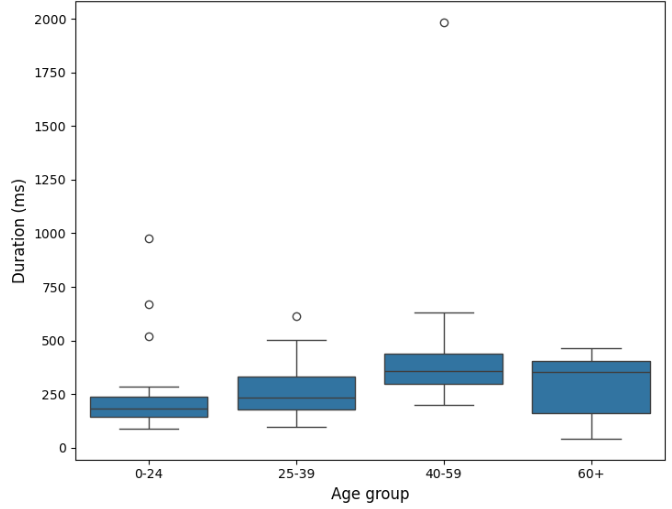
\includegraphics[width=13cm]{typing_speed.png}
    \caption{Box plot of keystroke interval of each age group.}
    \label{box_plot_typing_speed}
\end{figure}

During the processing of the data, keysrokes duration that took longer than five seconds are truncated.
This is done to remove data that is most likely caused by trivial factors, such as the user being away from keyboard.
Table \ref{tab:typing_behavior_one} shows the average and standard deviation of duration between each keystrokes after the data is truncated.

Age group 0-24 shows the fastest typing speed with an average keystroke interval of 241,54 ms.
This age group also shows the highest versatility in typing speed with a standard deviation of keystroke interval of 199,47 ms.

Age group 25-39 shows a slower typing speed than the previous age group.
This is, however, the second fastest typing speed with an average keystroke interval of 272,87 ms.
This age group is also the least variable in typing speed with a standard deviation of keystroke interval of 128,61 ms.

Age group 40-59 shows the slowest typing speed with an average keystroke interval of 386,99 ms.
This age group also shows high versatility in typing speed with a standard deviation of keystroke interval of 188,92 ms.

Average typing speed of age group 60+ increases compared to age group 40-59.
This age group has the second slowest typing speed with an average keystroke interval of 285,72 ms.

\begin{table}[h]
    \centering
    \begin{tabular}{ccccc}
    \toprule
    \multicolumn{1}{c}{} & \multicolumn{2}{c}{\textbf{Keystroke Interval}}\\
    \cmidrule(rl){2-3} \cmidrule(rl){4-5}
    \textbf{Age Group} & {Mean (ms)} & {Std. Dev (ms)} \\
    \midrule
    0-24 & 226.94 & 193.75 \\
    25-39 & 253.15 & 123.82  \\
    40-59 & 357.05 & 189.69 \\
    60+ & 279.32 & 132.83 \\
    \bottomrule
    \end{tabular}
    \caption{Keystroke interval of users in different age groups with truncation.}
    \label{tab:typing_behavior_one}
\end{table}

\begin{figure}[h!]
    \centering
    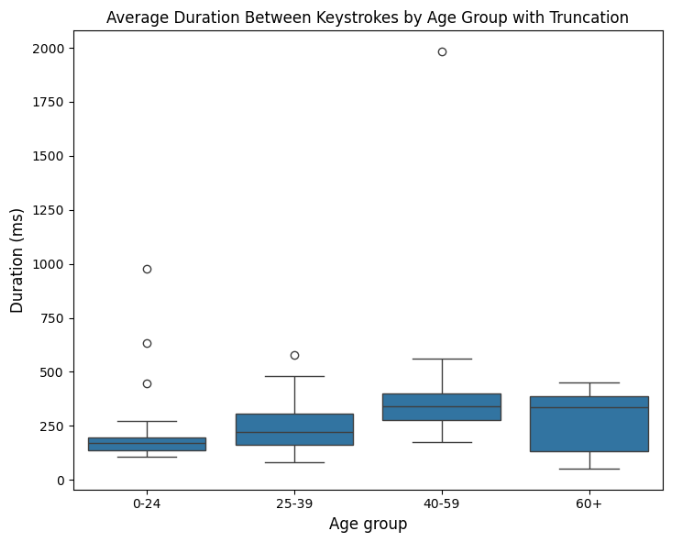
\includegraphics[width=13cm]{typing_speed_two_seconds.png}
    \caption{Box plot of keystroke interval of each age group with truncation of the one-percenth quantile.}
    \label{box_plot_typing_speed_two_seconds}
\end{figure}

Next, the data is truncated further by removing the one-percenth quantile (\textless1\% and \textgreater99\%) of the keystroke interval.
This is done to remove outliers from the data.
Table \ref{tab:typing_behavior_one} shows the average and standard deviation of duration between each keystrokes after data processing is done.

Age group 0-24 shows the fastest typing speed with an average keystroke interval of 226,94 ms.
Similar to the previous evaluation, this age group also shows the highest versatility in typing speed with a standard deviation of keystroke interval of 193,75 ms.

Age group 25-39 is slightly slower, with an average keystroke interval of 253,15 ms.
This is, however, still the second fastest typing speed.
This group also has the least variable typing speed with a standard deviation of keystroke interval of 123,82 ms.

Age group 40-59 has the slowest typing speed with an average keystroke interval of 357,05 ms.
Versatility in typing speed of this group is high with a standard deviation of keystroke interval of 189,69 ms.

For age group 60+ the average typing speed is slightly faster than age group 40-59.
This age group has the second slowest typing speed with an average keystroke interval of 279,32 ms.
Versatility in typing speed of this group is low with a keystroke interval of 132,83 ms.

\begin{table}[h]
    \centering
    \begin{tabular}{ccccc}
    \toprule
    \multicolumn{1}{c}{} & \multicolumn{2}{c}{\textbf{Keystroke Interval}}\\
    \cmidrule(rl){2-3} \cmidrule(rl){4-5}
    \textbf{Age Group} & {Mean (ms)} & {Std. Dev (ms)} \\
    \midrule
    0-24 & 195.69 & 117.00 \\
    25-39 & 253.84 & 121.98  \\
    40-59 & 344.07 & 82.60  \\
    60+ & 274.03 & 132.96 \\
    \bottomrule
    \end{tabular}
    \caption{Keystroke interval of users in different age groups with truncation based on \ac{IQR}.}
    \label{tab:typing_behavior_iqr}
\end{table}


\begin{figure}[h!]
    \centering
    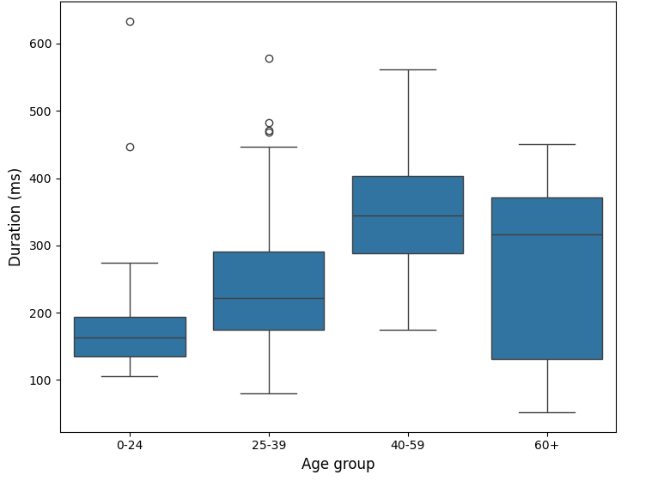
\includegraphics[width=13cm]{iqr.png}
    \caption{Box plot of keystroke interval of each age group with truncation based on \ac{IQR} method.}
    \label{box_plot_typing_speed_iqr}
\end{figure}

In this evaluation, the data is processed by removing the outliers (according to \ac{IQR} method) from data of duration between keystrokes.
This truncation is done after removing keystrokes that took longer than five seconds.
The ranking of the age groups in terms of average typing speed remains the same with the previous evaluation methods.
However, the ranking of the age groups in terms of versatility in typing speed changes.

Age group 0-24 that was previously the most variable in typing speed is now the second least variable with standard deviation of keystroke interval of 117 ms.
Age group 25-39 that was previously the least variable in typing speed is now the second most variable with standard deviation of keystroke interval of 121,98 ms.
Age group 40-59 that was previously the second most variable in typing speed is now the least variable with standard deviation of keystroke interval of 82,60 ms.
Lastly, age group 60+ that was previously the second least variable in typing speed is now the most variable with standard deviation of keystroke interval of 132,96 ms. 

\section{Findings}

% \textit{Note: Interpret the results and conclude interesting findings}
Backspace percentage average increases the older a person is, except for age group 60+.
A big jump in backspace percentage average is seen between age group 25-39 and 40-59 from 6.63\% to 15.93\%.
Afterwards, the backspace percentage average decreases to 3.29\% for age group 60+.

On all three evaluations, there is a noticeable pattern that the older the person is, the slower their typing speed become.
This is consistent with the general knowledge that the older a person is, the slower their reaction time is.
There is however an exception with age group 60+.
This group has a faster typing speed than age group 40-59 in all of the evaluations.
The fact that this group has the least amount of unique conversations might contribute to this result.

On the first two evaluations, i.e. evaluations without the \ac{IQR} method, if the data for age group 25-39 is left out, there is a trend where the older the age group, the less variable the typing speed is.
Age group 25-39 is, however, an exception to this pattern, as it is the least variable group.
In the evaluation with the \ac{IQR} method, this is reversed.
In this evaluation, exluding age group 40-59, the older a person is, the more variable their typing speed become.

\section{Limitations}

% \textit{Note: Describe limitations and threats to validity of your evaluation, e.g. reliability, generalizability, selection bias, researcher bias}
One of the limitations of the application that becomes apparent during the evaluation is the incapability of knowing whether the conversation is done by typing on the screen or with a physical keyboard.
Typing on a physical keyboard is generally faster than typing on a screen \cite{Varcholik2012}.
This is a limitation of the current version of the application.
Updating the application to also collect data of the device used while using the application should be considered in the future.
This will make sure that the data is more accurate and can be used to make more accurate conclusions.

Another limitation is the fact that the data is gathered from a specific group of people and the small sample size.
This specific group of people might not be representative of the general population, thus impacting the generalizability of the result.
The small sample size also makes the result less reliable.
To improve the reliability of the result, the application should be used by a larger group of people.
\chapter{Summary}

% \textit{Note: This chapter includes the status of your thesis, a conclusion and an outlook about future work.}

\section{Status}

% \textit{Note: Describe honestly the achieved goals (e.g. the well implemented and tested use cases) and the open goals here. if you only have achieved goals, you did something wrong in your analysis.}

The goal of developing a mobile-optimized chat application that collects the user's typing data has been achieved.
The application has been designed to be user-friendly for all age groups, specifically the elderly.
Clean architecture and secure coding practices have also been practiced to ensure reliability, scalability, and maintainability.
However, these characteristics could not be proofen yet and still subject to further testing and evaluation.
An improvenemt to the application could also be made by collecting data of the media used by the user.
This could improve the accuracy of the analysis of the data. 

\subsection{Realized Goals}

\textit{Note: Summarize the achieved goals by repeating the realized requirements or use cases stating how you realized them.}

\subsection{Open Goals}

\textit{Note: Summarize the open goals by repeating the open requirements or use cases and explaining why you were not able to achieve them. \textbf{Important:} It might be suspicious, if you do not have open goals. This usually indicates that you did not thoroughly analyze your problems.}

\section{Conclusion}

\textit{Note: Recap shortly which problem you solved in your thesis and discuss your \textbf{contributions} here.}

\section{Future Work}

\textit{Note: Tell us the next steps  (that you would do if you have more time. be creative, visionary and open-minded here.}

\appendix
\chapter{e.g. Questionnaire}

\textit{Note: If you have large models, additional evaluation data like questionnaires or non summarized results, put them into the appendix.}

\chapter{Tips for writing a thesis in TeX}

	\section{using this template}
		This template tries to achieve a separation of the template itself and the parts that are specific to the thesis. Ideally, the template does not have to be edited.

	The content of the thesis shall be added to the following files and folders:
	\begin{itemize}
		\item the \texttt{.tex}-files in the \texttt{chapters}-folder shall contain the description of your scientific work.
		\item the \texttt{.tex}-files in the \texttt{resources}-folder contain templates and examples, into which metadata, settings and organisational information about the thesis can be entered.
		\item the \texttt{thesis.bib}-file shall contain a list of the literature, that you cite in your thesis.
	\end{itemize}

	\section{General tips}
		Track your work on this thesis with a version control system such as git.

		In your TeX source code, use one line per sentence.
		This facilitates spotting excessively long sentences.
		Also, it makes the tracking of changes by the version control system more useful.
		If you add line breaks after a fixed number of columns instead, a change affects all subsequent lines of the paragraph, even though the actual contend has not been changed.

		It is recommended to create a folder, in which all images, that are included in this document are stored.
		See the \texttt{resources/settings.tex}-file, on how to add this folder to the default graphics path, so only the filenames have to be entered, when including an image.



	% Create lists of figures and tables
	\clearpage
	\listoffigures
	\clearpage
	\listoftables
	\clearpage

	% Include the bibliography
	\bibliography{thesis}
	\bibliographystyle{alpha}

\end{document}
